%%%%%%%%%%%%%%%%%%%%%%%%%%%%%%%%%%%%%%%%%%%%%%%%%%%%%%%%%%%%%%%
%% OXFORD THESIS TEMPLATE

% Use this template to produce a standard thesis that meets the Oxford University requirements for DPhil submission
%
% Originally by Keith A. Gillow (gillow@maths.ox.ac.uk), 1997
% Modified by Sam Evans (sam@samuelevansresearch.org), 2007
% Modified by John McManigle (john@oxfordechoes.com), 2015
% Modified by Ulrik Lyngs (ulrik.lyngs@cs.ox.ac.uk), 2018-, for use with R Markdown
%
% Ulrik Lyngs, 25 Nov 2018: Following John McManigle, broad permissions are granted to use, modify, and distribute this software
% as specified in the MIT License included in this distribution's LICENSE file.
%
% John commented this file extensively, so read through to see how to use the various options.  Remember that in LaTeX,
% any line starting with a % is NOT executed.

%%%%% PAGE LAYOUT
% The most common choices should be below.  You can also do other things, like replace "a4paper" with "letterpaper", etc.

% 'twoside' formats for two-sided binding (ie left and right pages have mirror margins; blank pages inserted where needed):
%\documentclass[a4paper,twoside]{templates/ociamthesis}
% Specifying nothing formats for one-sided binding (ie left margin > right margin; no extra blank pages):
%\documentclass[a4paper]{ociamthesis}
% 'nobind' formats for PDF output (ie equal margins, no extra blank pages):
%\documentclass[a4paper,nobind]{templates/ociamthesis}

% As you can see from the line below, oxforddown uses the a4paper size, 
% and passes in the binding option from the YAML header in index.Rmd:
\documentclass[a4paper, nobind]{templates/ociamthesis}


%%%%% ADDING LATEX PACKAGES
% add hyperref package with options from YAML %
\usepackage[pdfpagelabels]{hyperref}
% handle long urls
\usepackage{xurl}
% change the default coloring of links to something sensible
\usepackage{xcolor}

\definecolor{mylinkcolor}{RGB}{0,0,139}
\definecolor{myurlcolor}{RGB}{0,0,139}
\definecolor{mycitecolor}{RGB}{0,33,71}

\hypersetup{
  hidelinks,
  colorlinks,
  linktocpage=true,
  linkcolor=mylinkcolor,
  urlcolor=myurlcolor,
  citecolor=mycitecolor
}


% add float package to allow manual control of figure positioning %
\usepackage{float}

% enable strikethrough
\usepackage[normalem]{ulem}

% use soul package for correction highlighting
\usepackage{color, soulutf8}
\definecolor{correctioncolor}{HTML}{CCCCFF}
\sethlcolor{correctioncolor}
\newcommand{\ctext}[3][RGB]{%
  \begingroup
  \definecolor{hlcolor}{#1}{#2}\sethlcolor{hlcolor}%
  \hl{#3}%
  \endgroup
}
% stop soul from freaking out when it sees citation commands
\soulregister\ref7
\soulregister\cite7
\soulregister\citet7
\soulregister\autocite7
\soulregister\textcite7
\soulregister\pageref7

%%%%% FIXING / ADDING THINGS THAT'S SPECIAL TO R MARKDOWN'S USE OF LATEX TEMPLATES
% pandoc puts lists in 'tightlist' command when no space between bullet points in Rmd file,
% so we add this command to the template
\providecommand{\tightlist}{%
  \setlength{\itemsep}{0pt}\setlength{\parskip}{0pt}}
 
% allow us to include code blocks in shaded environments

% User-included things with header_includes or in_header will appear here
% kableExtra packages will appear here if you use library(kableExtra)
\usepackage{booktabs}
\usepackage{longtable}
\usepackage{array}
\usepackage{multirow}
\usepackage{wrapfig}
\usepackage{float}
\usepackage{colortbl}
\usepackage{pdflscape}
\usepackage{tabu}
\usepackage{threeparttable}
\usepackage{threeparttablex}
\usepackage[normalem]{ulem}
\usepackage{makecell}
\usepackage{xcolor}


%UL set section header spacing
\usepackage{titlesec}
% 
\titlespacing\subsubsection{0pt}{24pt plus 4pt minus 2pt}{0pt plus 2pt minus 2pt}


%UL set whitespace around verbatim environments
\usepackage{etoolbox}
\makeatletter
\preto{\@verbatim}{\topsep=0pt \partopsep=0pt }
\makeatother


%%%%%%% PAGE HEADERS AND FOOTERS %%%%%%%%%
\usepackage{fancyhdr}
\setlength{\headheight}{15pt}
\fancyhf{} % clear the header and footers
\pagestyle{fancy}
\renewcommand{\chaptermark}[1]{\markboth{\thechapter. #1}{\thechapter. #1}}
\renewcommand{\sectionmark}[1]{\markright{\thesection. #1}} 
\renewcommand{\headrulewidth}{0pt}

\fancyhead[LO]{\emph{\leftmark}} 
\fancyhead[RE]{\emph{\rightmark}} 




% UL page number position 
\fancyfoot[C]{\emph{\thepage}} %regular pages
\fancypagestyle{plain}{\fancyhf{}\fancyfoot[C]{\emph{\thepage}}} %chapter pages




%%%%% SELECT YOUR DRAFT OPTIONS
% This adds a "DRAFT" footer to every normal page.  (The first page of each chapter is not a "normal" page.)

% IP feb 2021: option to include line numbers in PDF

% for line wrapping in code blocks
\usepackage{fancyvrb}
\usepackage{fvextra}
\DefineVerbatimEnvironment{Highlighting}{Verbatim}{breaklines=true, breakanywhere=true, commandchars=\\\{\}}

% This highlights (in blue) corrections marked with (for words) \mccorrect{blah} or (for whole
% paragraphs) \begin{mccorrection} . . . \end{mccorrection}.  This can be useful for sending a PDF of
% your corrected thesis to your examiners for review.  Turn it off, and the blue disappears.
\correctionstrue


%%%%% BIBLIOGRAPHY SETUP
% Note that your bibliography will require some tweaking depending on your department, preferred format, etc.
% If you've not used LaTeX before, I recommend just using pandoc for citations -- this is what's used unless you specific e.g. "citation_package: natbib" in index.Rmd
% If you're already a LaTeX pro and are used to natbib or something, modify as necessary.

% this allows the latex template to handle pandoc citations
\newlength{\cslhangindent}
\setlength{\cslhangindent}{1.5em}
\newlength{\csllabelwidth}
\setlength{\csllabelwidth}{3em}
\newlength{\cslentryspacingunit} % times entry-spacing
\setlength{\cslentryspacingunit}{\parskip}
\newenvironment{CSLReferences}[2] % #1 hanging-ident, #2 entry spacing
 {% don't indent paragraphs
  \setlength{\parindent}{0pt}
  % turn on hanging indent if param 1 is 1
  \ifodd #1
  \let\oldpar\par
  \def\par{\hangindent=\cslhangindent\oldpar}
  \fi
  % set entry spacing
  \setlength{\parskip}{1mm}
  \setlength{\baselineskip}{6mm}
 }%
 {}
\usepackage{calc}
\newcommand{\CSLBlock}[1]{#1\hfill\break}
\newcommand{\CSLLeftMargin}[1]{\parbox[t]{\csllabelwidth}{#1}}
\newcommand{\CSLRightInline}[1]{\parbox[t]{\linewidth - \csllabelwidth}{#1}\break}
\newcommand{\CSLIndent}[1]{\hspace{\cslhangindent}#1}




% Uncomment this if you want equation numbers per section (2.3.12), instead of per chapter (2.18):
%\numberwithin{equation}{subsection}


%%%%% THESIS / TITLE PAGE INFORMATION
% Everybody needs to complete the following:
\title{\texttt{Feasibility\ and\ Acceptance\ of\ Chatbots\ Embedded\ in\ Healthcare\ Curricula}:}
\author{Matthew Pears}
\college{Research Fellow application}

% Master's candidates who require the alternate title page (with candidate number and word count)
% must also un-comment and complete the following three lines:

% Uncomment the following line if your degree also includes exams (eg most masters):
%\renewcommand{\submittedtext}{Submitted in partial completion of the}
% Your full degree name.  (But remember that DPhils aren't "in" anything.  They're just DPhils.)
\degree{January}

% Term and year of submission, or date if your board requires (eg most masters)
\degreedate{2023}


%%%%% YOUR OWN PERSONAL MACROS
% This is a good place to dump your own LaTeX macros as they come up.

% To make text superscripts shortcuts
\renewcommand{\th}{\textsuperscript{th}} % ex: I won 4\th place
\newcommand{\nd}{\textsuperscript{nd}}
\renewcommand{\st}{\textsuperscript{st}}
\newcommand{\rd}{\textsuperscript{rd}}

%%%%% THE ACTUAL DOCUMENT STARTS HERE
\begin{document}

%%%%% CHOOSE YOUR LINE SPACING HERE
% This is the official option.  Use it for your submission copy and library copy:
\setlength{\textbaselineskip}{22pt plus2pt}
% This is closer spacing (about 1.5-spaced) that you might prefer for your personal copies:
%\setlength{\textbaselineskip}{18pt plus2pt minus1pt}

% You can set the spacing here for the roman-numbered pages (acknowledgements, table of contents, etc.)
\setlength{\frontmatterbaselineskip}{17pt plus1pt minus1pt}

% UL: You can set the line and paragraph spacing here for the separate abstract page to be handed in to Examination schools
\setlength{\abstractseparatelineskip}{13pt plus1pt minus1pt}
\setlength{\abstractseparateparskip}{0pt plus 1pt}

% UL: You can set the general paragraph spacing here - I've set it to 2pt (was 0) so
% it's less claustrophobic
\setlength{\parskip}{2pt plus 1pt}

%
% Customise title page
%
\def\crest{{
\includegraphics[width=5cm]{templates/w.png}}}
\renewcommand{\university}{------------}
\renewcommand{\submittedtext}{}
\renewcommand{\thesistitlesize}{\fontsize{22pt}{28pt}\selectfont}
\renewcommand{\gapbeforecrest}{25mm}
\renewcommand{\gapaftercrest}{25mm
}


% Leave this line alone; it gets things started for the real document.
\setlength{\baselineskip}{\textbaselineskip}


%%%%% CHOOSE YOUR SECTION NUMBERING DEPTH HERE
% You have two choices.  First, how far down are sections numbered?  (Below that, they're named but
% don't get numbers.)  Second, what level of section appears in the table of contents?  These don't have
% to match: you can have numbered sections that don't show up in the ToC, or unnumbered sections that
% do.  Throughout, 0 = chapter; 1 = section; 2 = subsection; 3 = subsubsection, 4 = paragraph...

% The level that gets a number:
\setcounter{secnumdepth}{2}
% The level that shows up in the ToC:
\setcounter{tocdepth}{1}


%%%%% ABSTRACT SEPARATE
% This is used to create the separate, one-page abstract that you are required to hand into the Exam
% Schools.  You can comment it out to generate a PDF for printing or whatnot.

% JEM: Pages are roman numbered from here, though page numbers are invisible until ToC.  This is in
% keeping with most typesetting conventions.
\begin{romanpages}

% Title page is created here
\maketitle

%%%%% DEDICATION
\begin{dedication}
  Made in RMarkdown
\end{dedication}

%%%%% ACKNOWLEDGEMENTS


\begin{acknowledgements}
 	This work is supported by the ERASMUS+ Strategic Partnership in Higher Education ``Chatbot Enhance Personalise European Healthcare Curricula (CEPEH)'' (www.cepeh.eu) (2019-1-UK01- KA203-062091) project of the European Union.

 \begin{flushright}
 The CEPEH Team \\
 \end{flushright}
\end{acknowledgements}



%%%%% ABSTRACT


\renewcommand{\abstracttitle}{Abstract}
\begin{abstract}
	i will not duplicate the application but this rmarkdown allows report writing and structured presentations.

this is the abstract if we were writing a report.
\end{abstract}



%%%%% MINI TABLES
% This lays the groundwork for per-chapter, mini tables of contents.  Comment the following line
% (and remove \minitoc from the chapter files) if you don't want this.  Un-comment either of the
% next two lines if you want a per-chapter list of figures or tables.
\dominitoc % include a mini table of contents

% This aligns the bottom of the text of each page.  It generally makes things look better.
\flushbottom

% This is where the whole-document ToC appears:
\tableofcontents

\listoffigures
	\mtcaddchapter
  	% \mtcaddchapter is needed when adding a non-chapter (but chapter-like) entity to avoid confusing minitoc

% Uncomment to generate a list of tables:
\listoftables
  \mtcaddchapter
%%%%% LIST OF ABBREVIATIONS
% This example includes a list of abbreviations.  Look at text/abbreviations.tex to see how that file is
% formatted.  The template can handle any kind of list though, so this might be a good place for a
% glossary, etc.
% First parameter can be changed eg to "Glossary" or something.
% Second parameter is the max length of bold terms.
\begin{mclistof}{List of Abbreviations}{3.2cm}

\item[CEPEH]

Chatbot Enhance Personalised European Healthcare curricula

\item[HELM]

Health E-Learning and Media team

\item[RLO]

Reusable Learning Object

\item[ASPIRE]

Aims Storyboarding Production Implementation Release Evaluation

\item[NLP]

Natural Language Processing

\item[NLU]

Natural Language Understanding

\item[A.I]

Artificial Intelligence

\item[TAM]

Technology Acceptance Model

\item[SUS]

System Usability Scale

\item[CUQ]

Chatbot Usability Questionnaire

\item[HIG]

HELM is Great

\end{mclistof} 


% The Roman pages, like the Roman Empire, must come to its inevitable close.
\end{romanpages}

%%%%% CHAPTERS
% Add or remove any chapters you'd like here, by file name (excluding '.tex'):
\flushbottom

% all your chapters and appendices will appear here
\hypertarget{introduction}{%
\chapter*{Introduction}\label{introduction}}
\addcontentsline{toc}{chapter}{Introduction}

\adjustmtc
\markboth{Introduction}{}

\hypertarget{sec-background}{%
\section*{Background}\label{sec-background}}
\addcontentsline{toc}{section}{Background}

i wont repeat the application but i am sure you get the drift of the rmarkdown, to allow easier report writing for our work:

eg

\begin{enumerate}
\def\labelenumi{\arabic{enumi}.}
\item
  (Essential to the job)
  Demonstrable experience of working with extended reality technologies; *
\item
  For Leeds Hospitals Charity (LHC) I created a VR and PC Non-technical skills medical training application. See attached document ``NTS Summary Report'' for more details- which was the report submitted to the LHC December 2022.
\end{enumerate}

This resource is called an immersive Reusable Learning Object (iRLO). The design and development process followed a well- evidenced and effective framework called the ASPIRE framework. I performed everything from recordings and assets to the unity app, experimental setup and analysis, reporting/publishing etc.

\begin{enumerate}
\def\labelenumi{\arabic{enumi}.}
\setcounter{enumi}{1}
\tightlist
\item
  I spent 5 years on my PhD which involved how surgical trainees deploy their attention in virtual environments to cues relating to patient safety. I made a VR app in Unreal, and combined expert insight to assess and train undergraduate ODP trainees.
\end{enumerate}

\begin{enumerate}
\def\labelenumi{\arabic{enumi}.}
\setcounter{enumi}{2}
\tightlist
\item
  I worked on the CoViRR (Co-Creation of Virtual Reality Reusable E-Resources for European Healthcare Education) ERASMUS+ strategic partnership which co-created virtual reality reusable e-resources promoting innovative practices in digital era, by supporting current curricula and fostering open education. CoViRR intervened where current digital health training still lacks in solving many issue.
\end{enumerate}

----i can add graphs and do statistical analyses etc. take a look at \url{https://cepeh-analytics.netlify.app/} that i am just creating, and \url{https://helm-analytics.netlify.app/} which i am analysing 100,000+ data

\hypertarget{this-would-be-the-methods-section-etc-etc}{%
\chapter{this would be the methods section etc etc}\label{this-would-be-the-methods-section-etc-etc}}

\minitoc 

\hypertarget{procedure}{%
\section{Procedure}\label{procedure}}

\hypertarget{participants-etc-etc}{%
\section{Participants etc etc}\label{participants-etc-etc}}

\hypertarget{rmd-basics}{%
\chapter{Results}\label{rmd-basics}}

\minitoc 

\noindent

\hypertarget{introduction-1}{%
\section{Introduction}\label{introduction-1}}

Hi there, I thought to create this site using R, Github and a web builder just to show I have at least a basic understanding.

\begin{longtable}[]{@{}lr@{}}
\caption{Previous Chatbot Usage of Participants\\
}\tabularnewline
\toprule()
Previous\_Chatbot\_Usage & n \\
\midrule()
\endfirsthead
\toprule()
Previous\_Chatbot\_Usage & n \\
\midrule()
\endhead
1-4 hours & 15 \\
10-19 hours & 1 \\
20+ hours & 1 \\
5-9 hours & 2 \\
Never & 23 \\
\bottomrule()
\end{longtable}

In short, approximately 50\% had never used a chatbot, and 45\% had used a
chatbot, at some period over the years, for a short period of time.

Most learners use books or online books as resources. They may use multiple sources however they were asked to note the primary source. Only 6 stated their primary sources were \emph{Online videos/interactive materials} which includes such tools as chatbots.

\begin{figure}
\centering
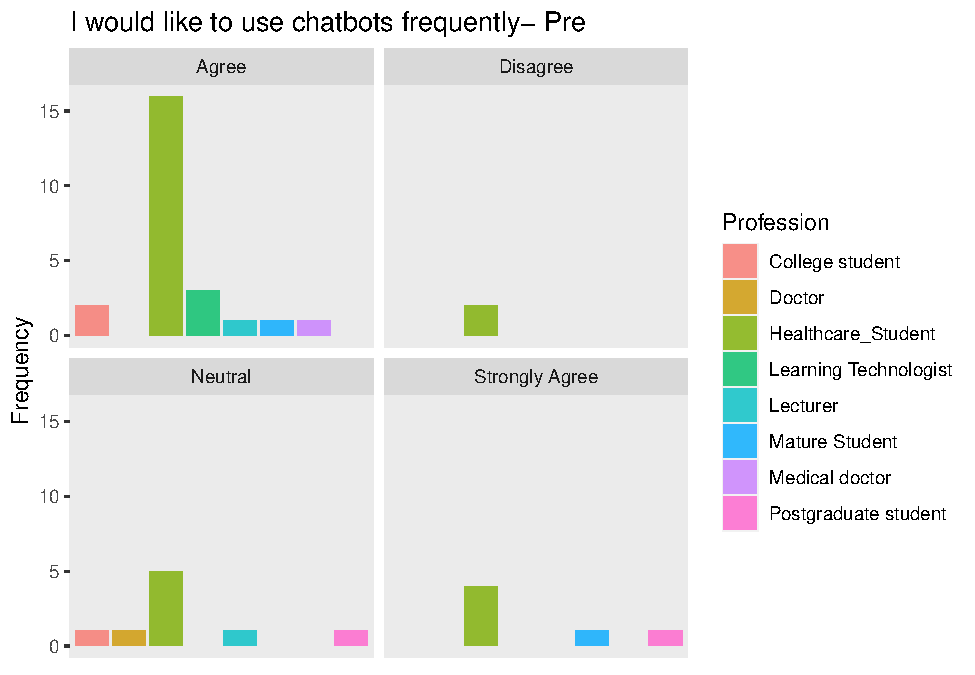
\includegraphics{_main_files/figure-latex/Boxplotsplits2-1.pdf}
\caption{\label{fig:Boxplotsplits2}Chatbot Usage agreements- Pre}
\end{figure}

The first boxplot (\ref{fig:Boxplotsplits2}) shows the intention, or at least the learners interest in using chatbots by means of agreeing that they would like to use chatbots if they had the opportunity. 20 healthcare students agreed (16) and strongly agreed (4) which made about 50\% of participants. 9 were neutral with 1 disagree.

\begin{figure}
\centering
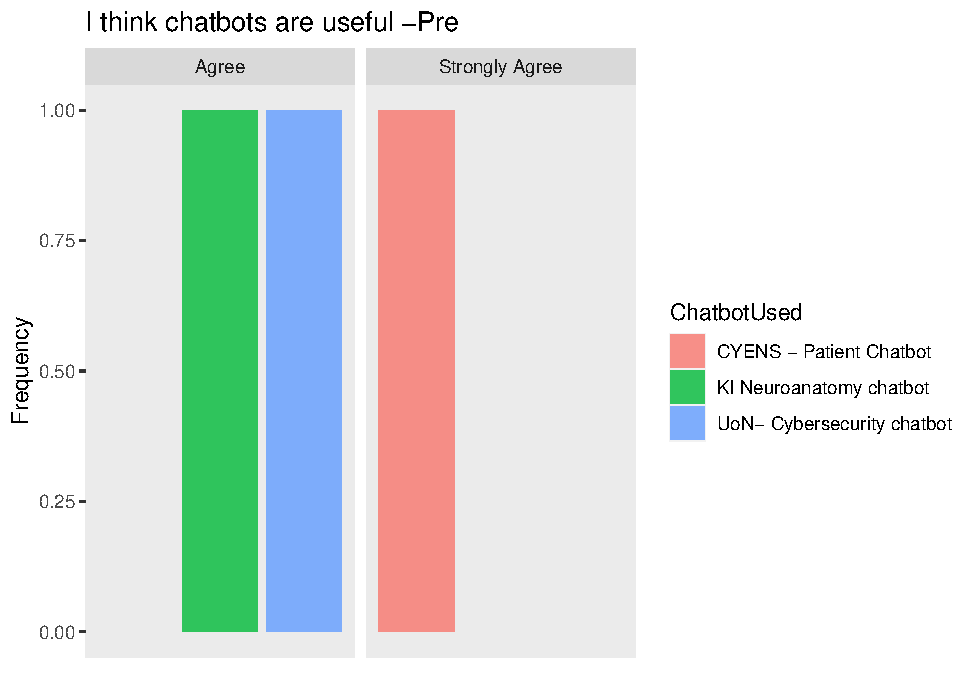
\includegraphics{_main_files/figure-latex/BoxplotUsefulPre-1.pdf}
\caption{\label{fig:BoxplotUsefulPre}Chatbots are Useful Opinion- Pre}
\end{figure}

(\ref{fig:BoxplotUsefulPre}) shows the opinions of all participants on the usefulness of chatbots. Many had not had experience with them yet had positive rating.

This positive opinions of chatbots may be from colleagues, friends, media, tutors, or other social information of the benefits in healthcare education. Around 25\% were neutral or disagreed that healthcare chatbots were useful.

\textbf{\emph{The participants then used the 4 chatbots and completed the post-usage survey after each chatbot. Results after use are as followed:}}

\hypertarget{chatbot-usability-questionnaire-cuq}{%
\section{Chatbot Usability Questionnaire (CUQ)}\label{chatbot-usability-questionnaire-cuq}}

\hypertarget{cuq-calculation-tool}{%
\subsection{CUQ Calculation tool}\label{cuq-calculation-tool}}

The CUQ was developed by researchers at Ulster University,
\href{https://www.ulster.ac.uk/research/topic/computer-science/artificial-intelligence/projects/cuq}{Link}
and as the calculation can be complex, a dedicated calculation tool has been created.

Please download the CEPEH CUQ calculation tool which has all of the data entered, so you can see the CEPEH CUQ scoring

\href{CUQ-Calculation-Tool.xlsx}{Click here to download CUQ calc tool}

\href{cuq.png}{Click here to download CEPEH CUQ score result}

\begin{figure}

{\centering 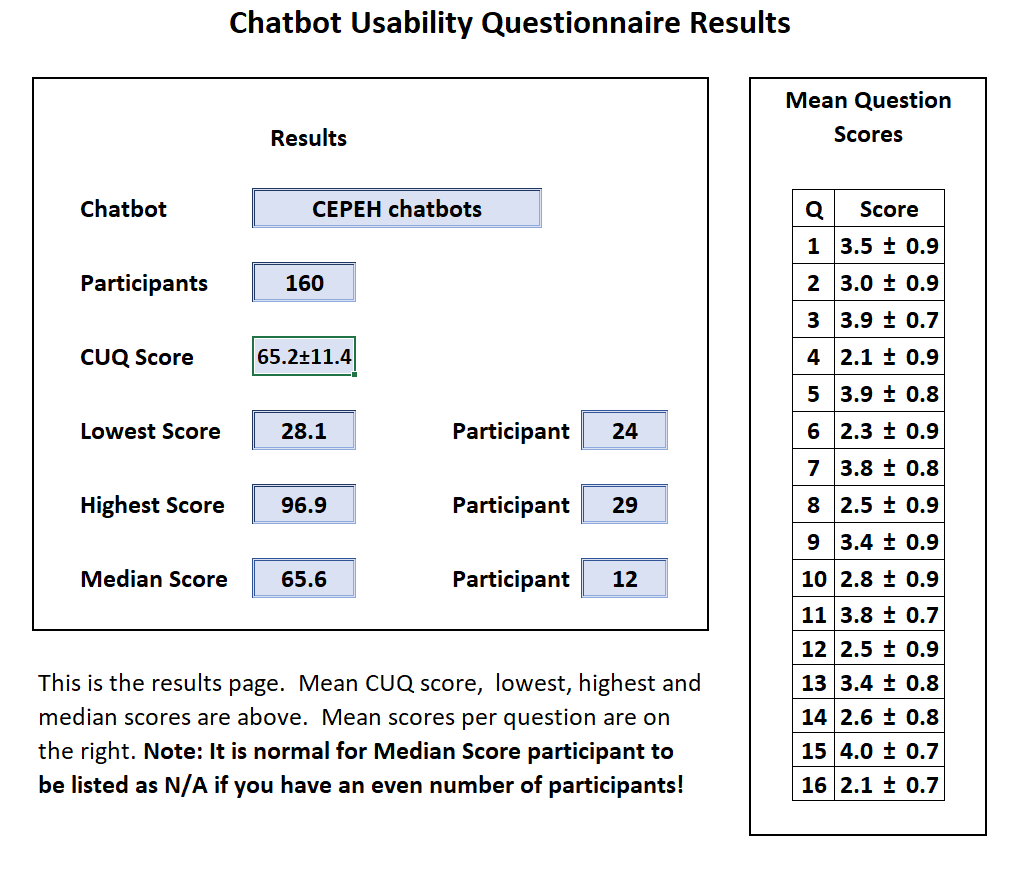
\includegraphics[width=0.75\linewidth]{cuq} 

}

\caption{CUQ CEPEH Score}\label{fig:cuqimage}
\end{figure}

Although the design and development was similar, each chatbot CUQ score was calculated to understand how the topic content may affect usability:

The breakdown of the chatbots was:

\begin{itemize}
\tightlist
\item
  Aristotle University of Thessaloniki CUQ score = 63/100
\item
  CYENS Centre of Excellence CUQ score = 67/100
\item
  Karolinska Institute CUQ score = 63/100
\item
  University of Nottingham CUQ score = 68/100
\end{itemize}

The score for all 3 chatbots grouped was 65/100. See Discussion CUQ
section for interpretation

\begin{figure}

{\centering 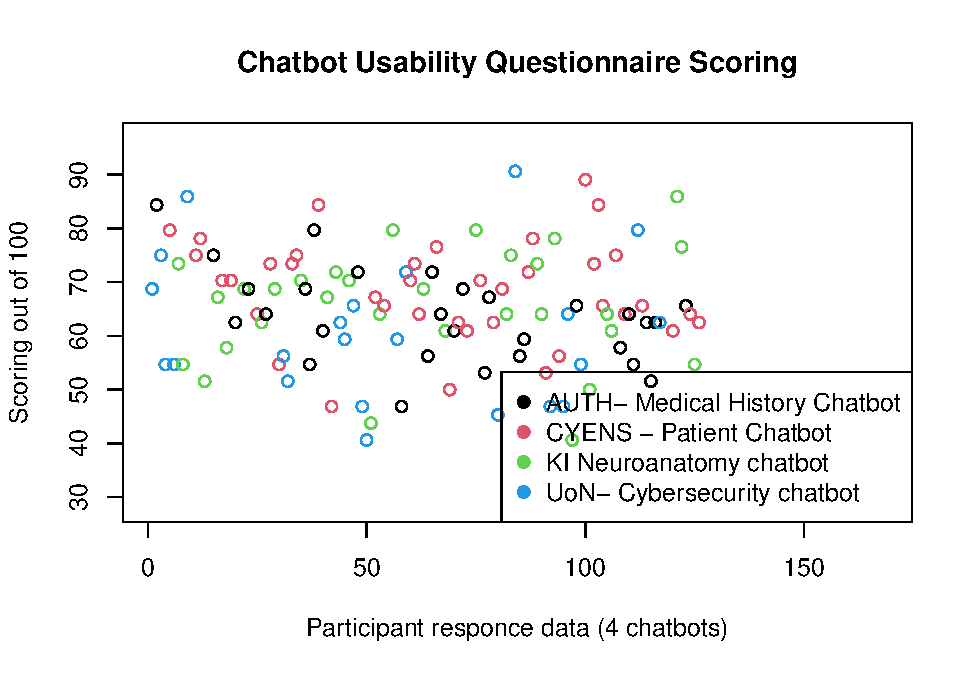
\includegraphics{_main_files/figure-latex/CUQscatterplot-1} 

}

\caption{CUQ Scatter Plot}\label{fig:CUQscatterplot}
\end{figure}

Figure (\ref{fig:CUQscatterplot}) shows the CUQ scores as a scatter plot to highlight how there was a moderate distribution of results.
Further exploration is required to understand which elements are causing this spread, and if it was due to problems within a small group of learners.

\hypertarget{system-usability-scale-sus-questions}{%
\section{System Usability Scale (SUS) Questions}\label{system-usability-scale-sus-questions}}

\emph{Note= The amount of `agreement' is defined as the addition of `Agree'
and `Strongly agree' responses.}

The SUS score should consist of 10 items. However, some SUS questions were improved upon by 1 or more CUQ questions, specifically to this Chatbot study. The SUS results would be obscured by the CUQ scores, expect 2 that did not have cross-over. The two questions were:

\begin{itemize}
\item
  I would like to use the CEPEH chatbot I tested, more frequently
\item
  I felt confident using the CEPEH chatbot
\end{itemize}

This meant the score of the SUS was not created, however the CUQ score better represented the Learners' perceptions of the CEPEH chatbot in terms of feasibility of use and acceptability in healthcare curricula.

\begin{longtable}[]{@{}lr@{}}
\toprule()
Keep Using CEPEH Chatbot & Responses \\
\midrule()
\endhead
Agree & 66 \\
Disagree & 15 \\
Neutral & 17 \\
Not Applicable & 3 \\
Strongly Agree & 23 \\
Strongly Disagree & 2 \\
\bottomrule()
\end{longtable}

The table \ref{tab:SUSkeepusing} above shows the results for agreement participants may
continue to use the CEPEH chatbots: 89/126 (70\%) agreed or strongly agreed. However, there were 23 records that learners were neutral or disagree they would continue use.

\begin{longtable}[]{@{}lr@{}}
\toprule()
Confidence using CEPEH Chatbot(s) & Responses \\
\midrule()
\endhead
Agree & 71 \\
Disagree & 11 \\
Neutral & 21 \\
Not Applicable & 4 \\
Strongly Agree & 19 \\
\bottomrule()
\end{longtable}

Confidence when using the chatbots is in table (\ref{tab:confidence})- it shows the distribution of agreement for participants for all
4 chatbots. The table shows 90/126 records that participants feel they are confident in using the chatbots. However, 21/126 (16\%) were neutral and 11/126 (8.5\%) disagreed and this was explored in the qualitative analysis section.

\hypertarget{technology-acceptance-model}{%
\section{Technology Acceptance Model}\label{technology-acceptance-model}}

The TAM questions were analysed according to their subsets. The subsets
were Perceived Usefulness (PU) and Perceived Ease of Use (PEU)

The questions were-

Perceived Usefulness (PU):
1. Using CEPEH chatbots would enable me to accomplish tasks more
quickly
2. Using CEPEH chatbots would increase performance
3. Using CEPEH chatbots would increase my productivity
4. I would find CEPEH chatbots useful on my course

Perceived Ease of Use (PEU):
5. Learning to use CEPEH chatbots would be easy to me
6. It would be easy for me to be skilful at using CEPEH chatbots
7. My interactions with CEPEH chatbots would be clear and understandable
8. I would find CEPEH chatbots easy to use

The scores as a percentage of agreement, were calculated by averaging the subsets and interpreted as:

\begin{itemize}
\item
  Before using the CEPEH chatbots, there was 66\% (2.2/5) agreement for the Perceived Usefulness of chatbots in healthcare education, and after 48\% (2.6/5) agreed.
\item
  Before using the CEPEH chatbots, there was 64\% (2.3) agreement for Perceived Ease of Use of chatbots in healthcare education, and after 51\% (2.56) agreed.
\end{itemize}

The justification for this may be due to being early versions of applications with limited functionality and functions which can be difficult for user to experience the intended further range of features and learning exercises.

\hypertarget{knowledge-and-trust-after-use}{%
\subsection{Knowledge and Trust after Use}\label{knowledge-and-trust-after-use}}

CYENS chatbot had around 10 more participants stating that they were neutral on gaining knowledge of the topic. The figure 2.6 shows the ratings by participants of the CEPEH Chatbots to provide them with the necessary course information.

\begin{figure}

{\centering 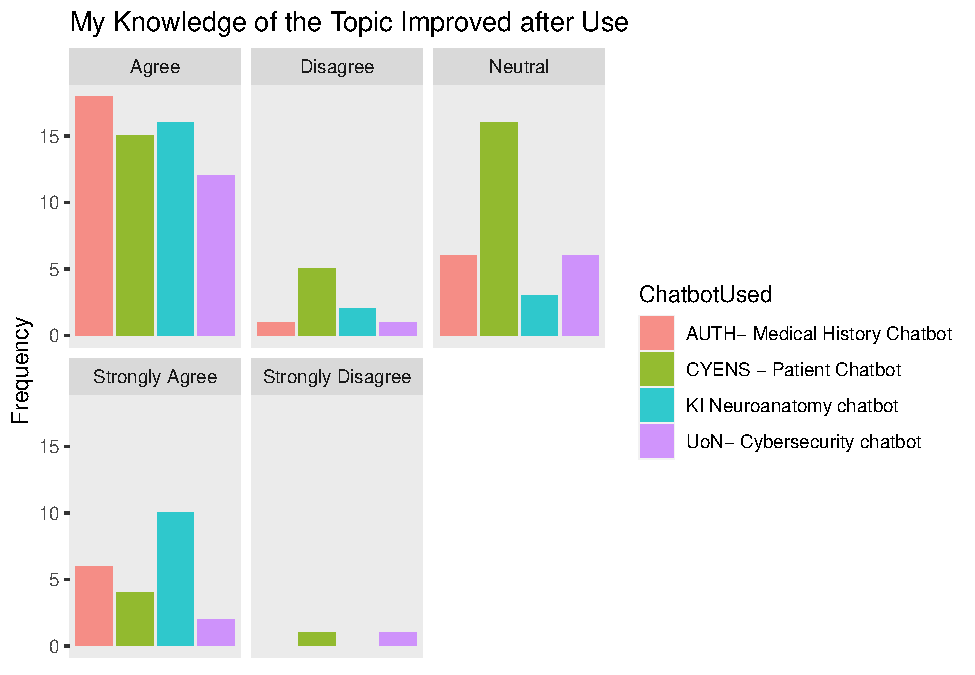
\includegraphics{_main_files/figure-latex/Boxplot knowledge-1} 

}

\caption{Improvements in Knowledge}(\#fig:Boxplot knowledge)
\end{figure}

The figure (@ref(fig:Boxplot trust)) shows the ratings by participants of the CEPEH Chatbots to provide them with the necessary course information.

\begin{figure}

{\centering 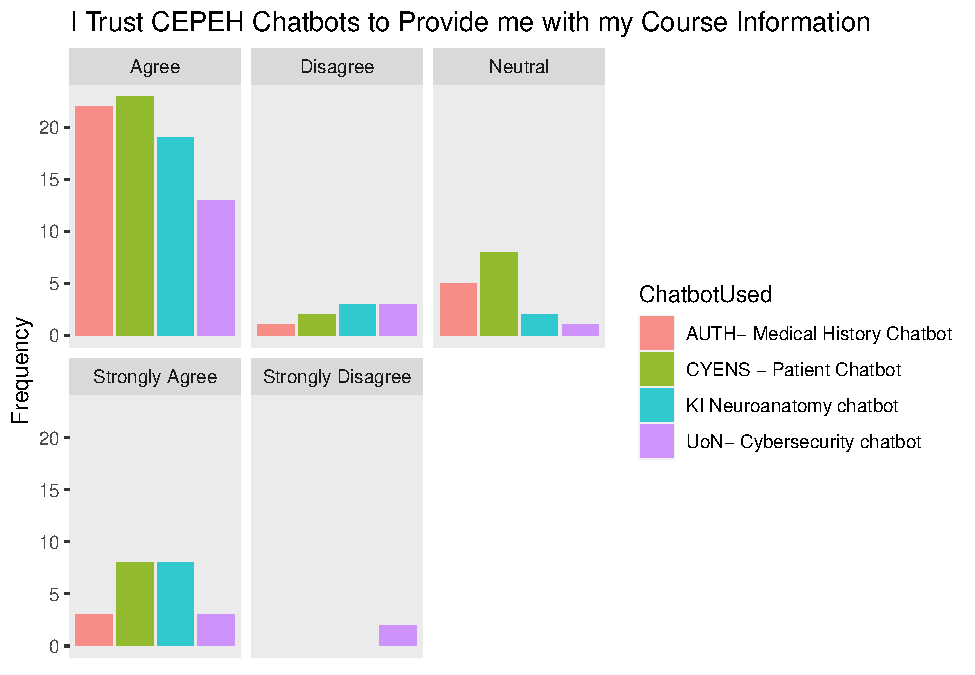
\includegraphics{_main_files/figure-latex/Boxplot trust-1} 

}

\caption{Trust Chatbots POST use}(\#fig:Boxplot trust)
\end{figure}

This is a integral element in learners' motivational and educational choices to reuse the learning resources. As previously described, the trust of the information is also a factor in these responses.

\hypertarget{personality-and-interactions}{%
\section{Personality and Interactions}\label{personality-and-interactions}}

\begin{center}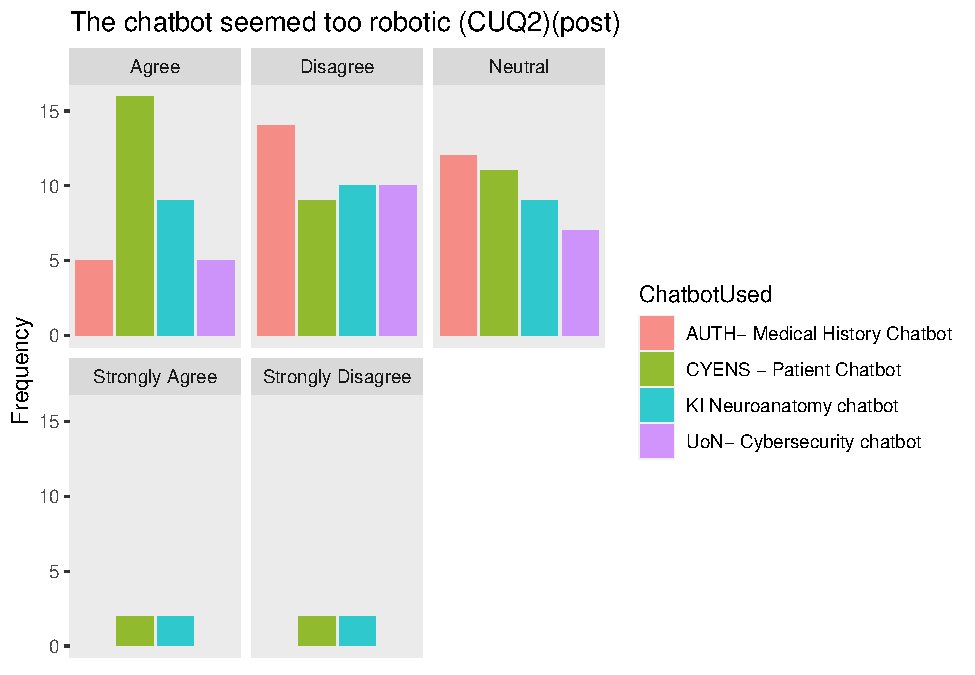
\includegraphics{_main_files/figure-latex/Boxplotsplits8-1} \end{center}

\emph{The chatbot seemed too robotic} results had the largest mix of
responses, and for all 4 chatbots evaluated. The University of
Nottingham Cybersecurity chatbot had more deterministic pathways with
exploitation of the NLP modelling to provide illusion of realism. This
may explain why there was less agreement. However, Neutrality and/or
agreement was not desired.

\begin{center}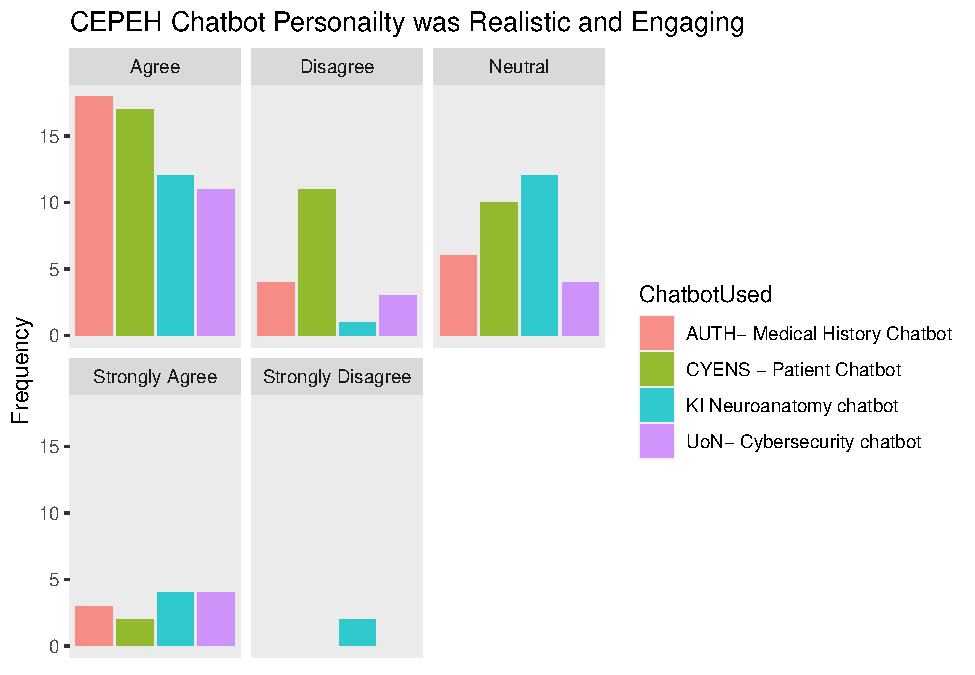
\includegraphics{_main_files/figure-latex/Boxplot personality-1} \end{center}

There were mixed results for the chatbot used being realistic and engaging. This question has two descriptive terms however based on the other results we understand that the chatbots' NLP logic, or ability to respond required improvement to be more `smooth' in replying. The primary limitation was found in the `robotic' interactions (See Figure x). This was
investigated further in the `Text Mining' and `Sentiment Analysis' sections.

\hypertarget{ease-of-use-and-seeking-support}{%
\section{Ease of Use and Seeking Support}\label{ease-of-use-and-seeking-support}}

\begin{figure}

{\centering 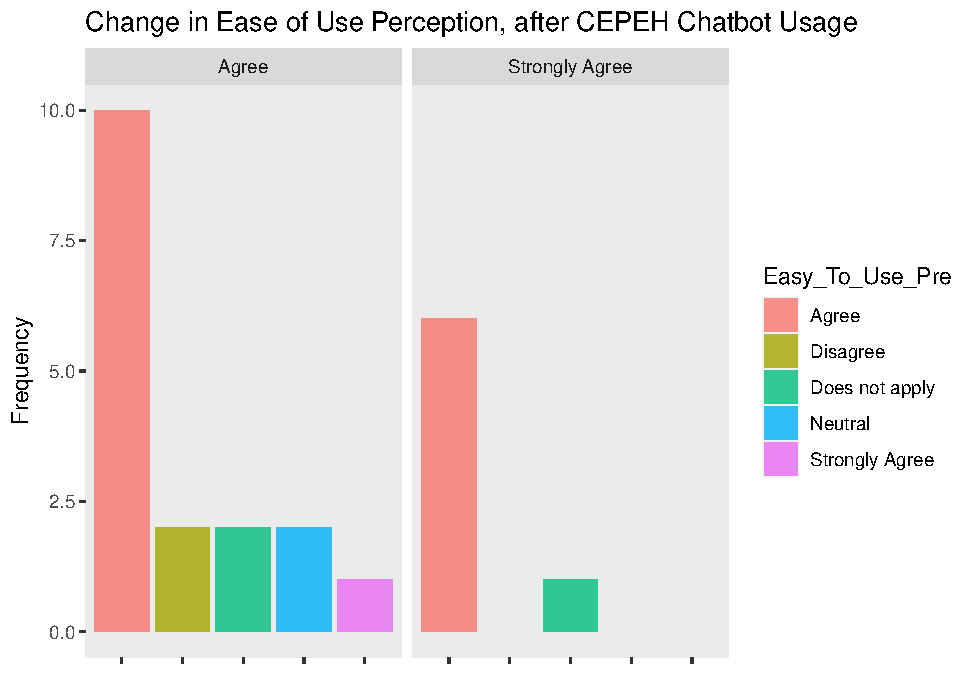
\includegraphics{_main_files/figure-latex/Boxplotsplits9-1} 

}

\caption{Ease of Use Comparison}\label{fig:Boxplotsplits9}
\end{figure}

After usage, there was only agreement in Ease of Use- as shown in
(\ref{fig:Boxplotsplits9} as there are no `Neutral' or disagree
columns. Any learners with disagreement before using the CEPEH chatbots,
after believed they were easy to use.

\begin{figure}
\centering
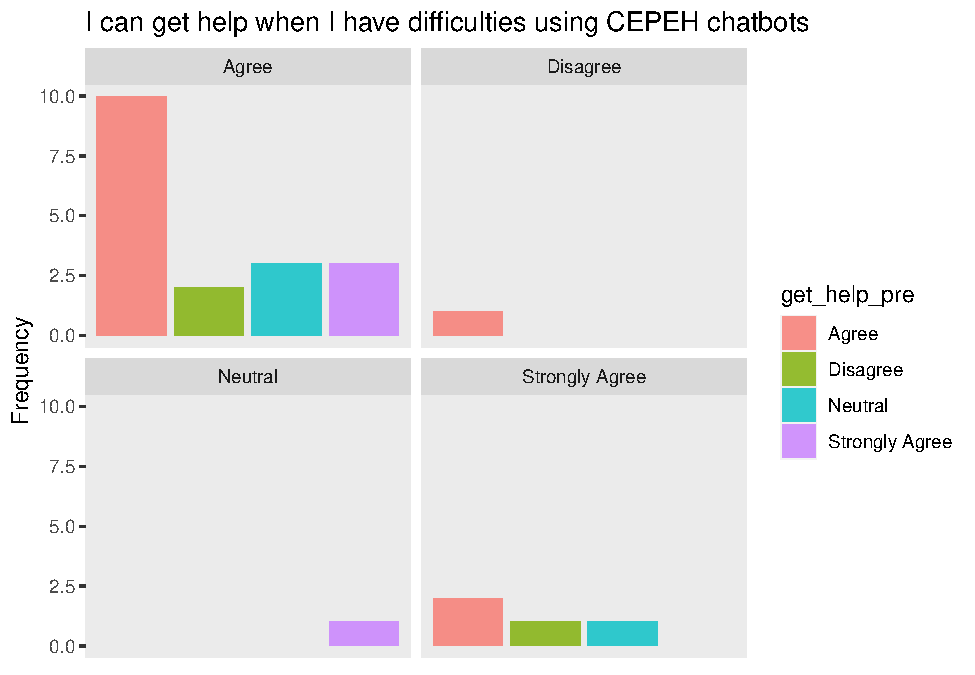
\includegraphics{_main_files/figure-latex/Boxplotsplits10-1.pdf}
\caption{\label{fig:Boxplotsplits10}Ease of Use Comparison}
\end{figure}

Those who disagreed or were neutral in the pre usage measure, improved
their understanding that help was available with the CEPEH chatbots.
After usage, 40 participants agreed they could get help if they had
difficulty using the resources.

\begin{figure}

{\centering 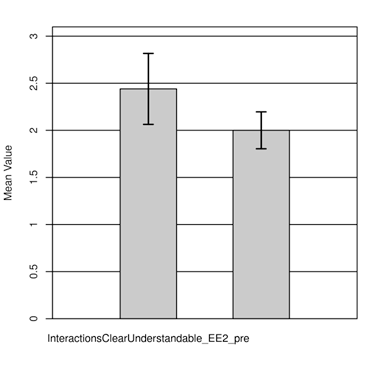
\includegraphics[width=5.33in]{clear} 

}

\caption{Pre-post accomplish quickly}\label{fig:accomplishquickly}
\end{figure}

\begin{figure}

{\centering 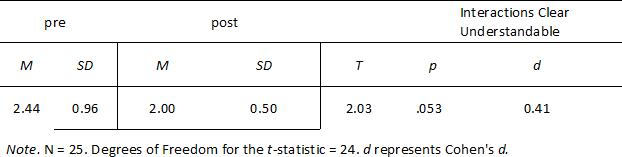
\includegraphics[width=8.64in]{table ttest} 

}

\caption{Table of T-test results}\label{fig:ttest}
\end{figure}

\begin{figure}

{\centering 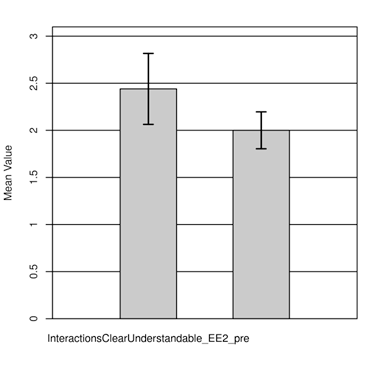
\includegraphics[width=5.33in]{clear} 

}

\caption{pre-post clear}\label{fig:clearpic}
\end{figure}

\begin{figure}

{\centering 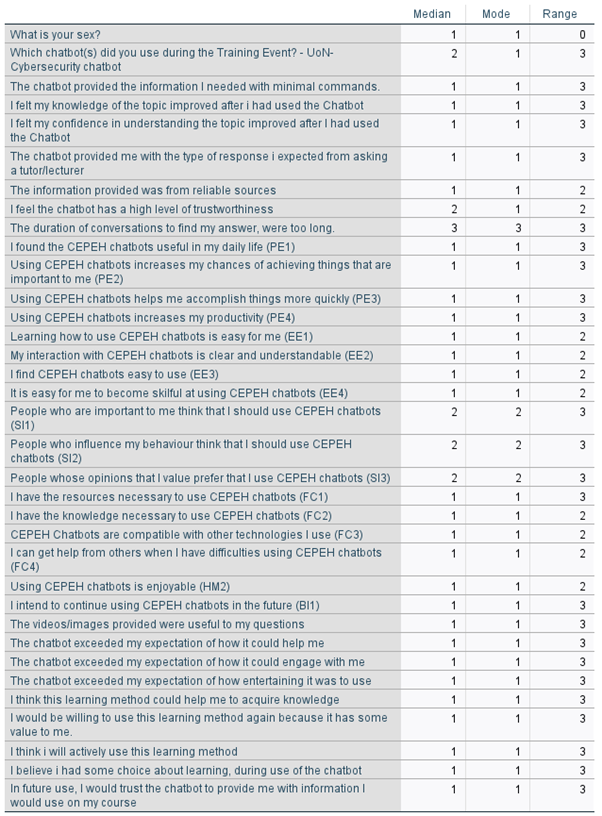
\includegraphics[width=10.19in,height=1.25\textheight]{bigtable} 

}

\caption{Table of Results}\label{fig:bigtable}
\end{figure}

This rather large table presents all of the descriptive statistic measures AFTER chatbot usage. The Mode is important to show that the majority of participants stated their perceptions, experience, and acceptance increased.

\hypertarget{inferential-statistics}{%
\section{Inferential Statistics}\label{inferential-statistics}}

Paired t-test involves matching the same participants on a variable before intervention with, ideally, the equal measure of variable after intervention. For this study, we used several metrics from the various questionnaires to facilitate pre-post comparisons. The CUQ was only asked after chatbot usage, however most other questions were able to have a pre-post comparison.

Importantly, there is value in the modes which indicate majority consensus, rather than mean driven t-tests. Being an initial single session with technical orientation for Users as well as practical usage, there is high change that a minority will experience technical or functional problems. Although the majority may benefit, the measures from this minority can significantly impact the measures. For example, if a sample of 42 have the results 5/5 (27), 4/5 (11), and 1/5 (5), the mode and median are 5 however the mean is 4.38. This can affect parametric or non-parametric results that infer equal experience from participant. We are not overlooking participants but factoring in their experiences as a minority and assessing their results in other ways- i.e., the focus group discussions. This better reflects each participants experience and the accuracy of efficacy of the chatbots.
Because of the experimental set-up and the 4 different chatbots, the meaning of the t-tests has small power and effect size. We intended for all metrics to improve, but to have significant findings with the setup does not provide much more information in addition to increased means/scores. We performed paired t-tests, however many paired samples had significant Shapiro-Wilk results indicating the normality assumption were violated. The test is robust to violations, and the same participants are being tested over Time, rather than different participants. This also indicated that the meaning of the Wilcoxon has limited strength.

\hypertarget{paired-sample-t-test-and-wilcoxon-signed-rank-test}{%
\subsection{Paired sample t-test and Wilcoxon signed rank test}\label{paired-sample-t-test-and-wilcoxon-signed-rank-test}}

Two-tailed paired t-tests were conducted to examine whether the mean difference is of the following groups were significantly different:

• Confidence
• Daily usefulness
• Increasing achievements
• Accomplishing things quickly
• Increased productivity
• Ease of use
• Clear and understandable interactions
• Use chatbots more frequently

The results showed there were no significant differences in these comparisons. For each comparison the results were:

• Confidence- t(24) = -0.35, \textbf{p = .731} (prem=1.96, postm=2.04)

• Daily usefulness- V = 48.50, z = -0.27, \textbf{p = .790} (prem=2.04, postm=2.12)

• Increasing achievements- t(24) = -0.18, \textbf{p = .857} (prem=2.28, postm=2.32)

• Accomplish tasks quickly- V = 36.00, z = -0.25, \textbf{p = .805} (prem=2.12, postm=2.16)

• Increased productivity- V = 96.00, z = -1.51, \textbf{p = .131} (prem=2.6, postm=2.24)

• Ease of use- V = 72.00, z = -1.32, \textbf{p = .186} (prem=2.36, postm=2.12)

• Clear and understandable interactions- V = 101.50, z = -1.82, \textbf{p = .068} (prem=2.2, postm=2.61)

• Use chatbots more frequently- t(24) = 0.45, \textbf{p = .657} (prem=2.2, postm=2.08)

As predicted, the sensitivity of the t-test meant Wilcoxon test was more appropriate for some measures. The results show minor increases in means for most, but minor decreases in others. These results have high standard deviations which are from a minority of participants scoring low, and explored in the focus group discussions.

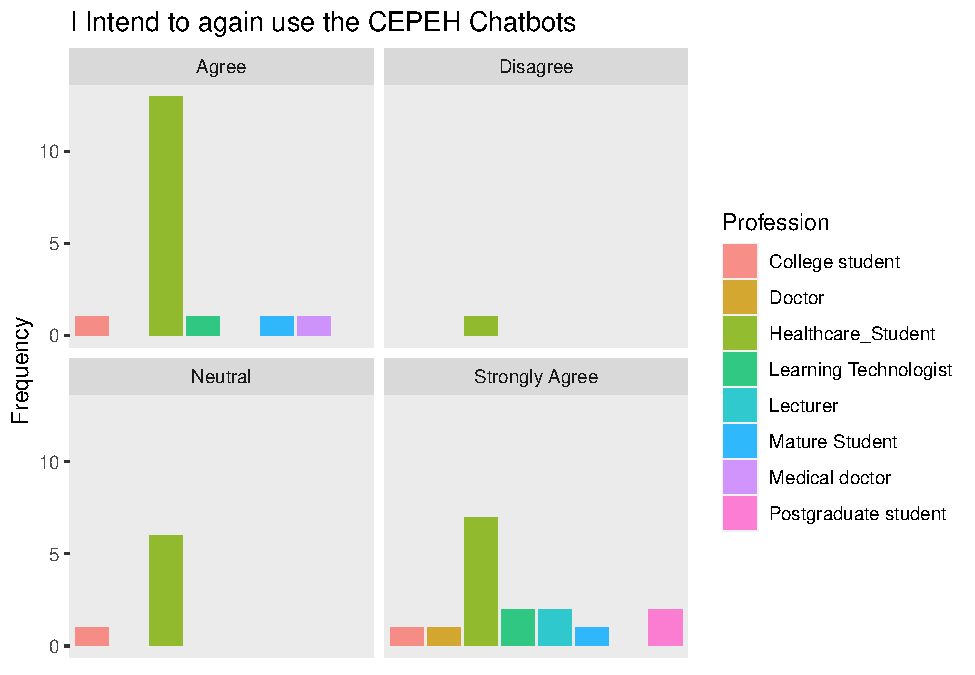
\includegraphics{_main_files/figure-latex/Boxplotsplits11-1.pdf}
After using the CEPEH chatbots, majority of participants stated they
would reuse the chatbots. However, there was 6 counts of \emph{disagree} or
\emph{strongly disagree} for all 4 chatbots. Further, there were 17 counts of
neutral in reuse, which was approximately 4 participants per chatbot
(see (\ref{fig:Boxplotsplits4}).

\begin{figure}
\centering
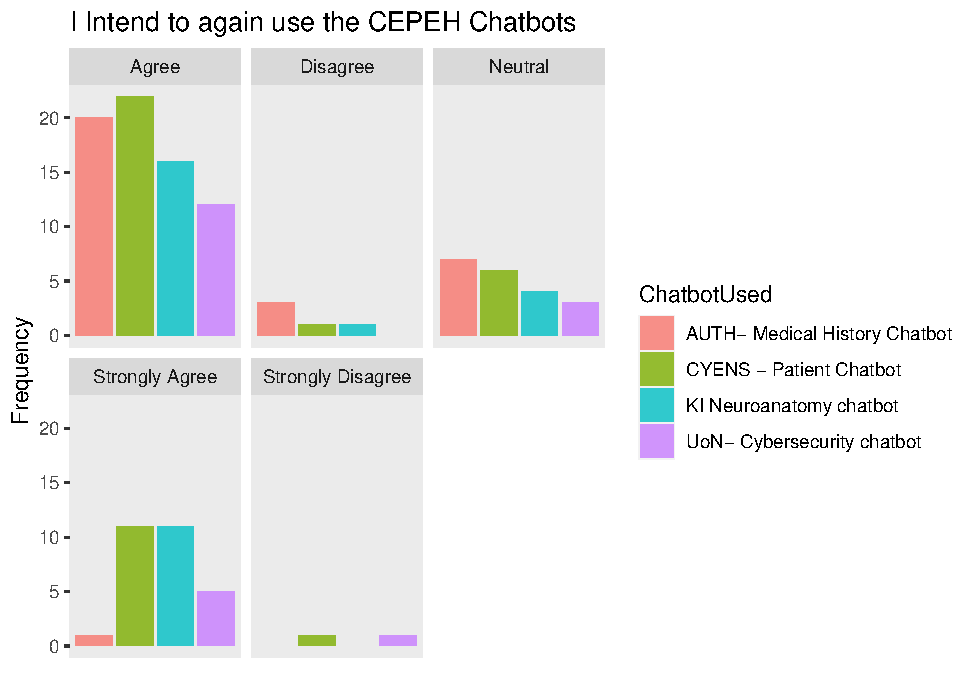
\includegraphics{_main_files/figure-latex/Boxplotsplits4-1.pdf}
\caption{\label{fig:Boxplotsplits4}Intend to Reuse-Post}
\end{figure}

For CYENS, even though the knowledge of the topic was not perceived to
improve by some participants, this box plot shows how 34/42 stated they
would reuse the chatbot developed by CYENS.

\begin{figure}
\centering
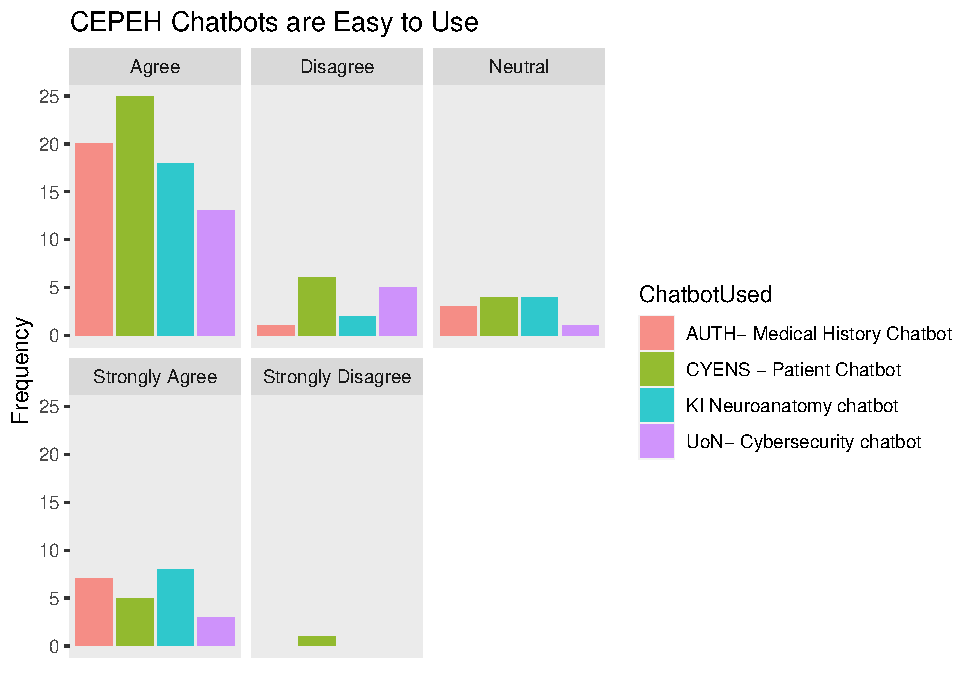
\includegraphics{_main_files/figure-latex/Boxplotsplits3-1.pdf}
\caption{\label{fig:Boxplotsplits3}Easy to Use- Post}
\end{figure}

There was only 1 `Strongly Disagree' response. The agreement options
counted for the majority of the data.
Repeated Measures t-test, aka paired t-test (before and after
measurements)

This t-test compares confident using mobile chatbots before and after
CEPEH chatbot usage.

\begin{center}\rule{0.5\linewidth}{0.5pt}\end{center}

output:
bookdown::pdf\_document2:
template: templates/template.tex
bookdown::html\_document2: default
bookdown::word\_document2: default
documentclass: book
\#bibliography: {[}bibliography/references.bib, bibliography/additional-references.bib{]}
editor\_options:
markdown:
wrap: 72
\# Text Mining, Natural Language Processing, and Sentiment Analysis
---

\hypertarget{and-here-is-a-bit-of-text-mining-i-am-doing-basic-frequency}{%
\chapter{and here is a bit of text mining i am doing, basic frequency}\label{and-here-is-a-bit-of-text-mining-i-am-doing-basic-frequency}}

The focus group discussions provided a lot of feedback for how the
participants experienced their interactions with the chatbots, and how
the CEPEH team can improve them, improve the design and development
processes, and improve uptake and sharing.

One method of analysing this data is with use of text mining and data
manipulation, creating word clouds, sentiment analysis, and using a
model which can distinguish the unique themes in text, and highlights
for us what text is used to create these themes.

Therefore, we have created a model to allow efficient and intelligent
analysis of this open/free focus group data.

\hypertarget{tokenising}{%
\section{Tokenising}\label{tokenising}}

Firstly, we tokenised the words from the FGDs. A Token is ``a meaningful
unit of text, most often a word, that we are interested in using for
further analysis''. For each word we give it a property that we can call
upon later.

The data manipulation for this included removing punctuation, converting
to lower-case, and setting word type to word (and not such types as
``characters'', ``ngrams'', ``sentences'', ``lines'' etc)

\hypertarget{stop-words}{%
\subsection{Stop words}\label{stop-words}}

The model then removed words with meaningless function. These are called
stop words. Words like ``the'', ``of'' and ``to'' are the most frequent words
found, technically, but are of little interest to us.

We also created a custom list of stop words for CEPEH. We know
participants may mention other objects, and the list was as followed:
found; chatbot; chatbots; presentation.

The data was ready for analysis by the model. We ordered it to find the
most frequent words. Below is a table with the 6 frequently occurring
words, showing how Stop words have now been filtered.

\begin{longtable}[]{@{}lr@{}}
\toprule()
word & n \\
\midrule()
\endhead
information & 11 \\
helpful & 8 \\
understand & 8 \\
idea & 7 \\
ideas & 7 \\
lot & 7 \\
\bottomrule()
\end{longtable}

This word list can then be used for sentiment analysis, (see \emph{Sentiment
Analysis} section), in addition to frequency of words.

\hypertarget{plotting-word-frequencies---bar-graphs}{%
\section{Plotting word frequencies - bar graphs}\label{plotting-word-frequencies---bar-graphs}}

\hypertarget{normalised-frequency}{%
\subsection{Normalised frequency}\label{normalised-frequency}}

With this information a list of top words from the participants in the
FGD can be rendered and after some modifications, a graph of the top 20
words is produced, with better aesthetics. This is a better way to
understand this data, and the axis can be normalised for the frequency
of occurrences in accordance with the source text. The raw text had 2827
words in total. Therefore we can mutate the ratios to reflect this.

\hypertarget{plotting-normalised-frequency}{%
\subsection{Plotting normalised frequency}\label{plotting-normalised-frequency}}

Now we can plot, for example, the 20 most frequent words when normalised
by the source text.

\begin{center}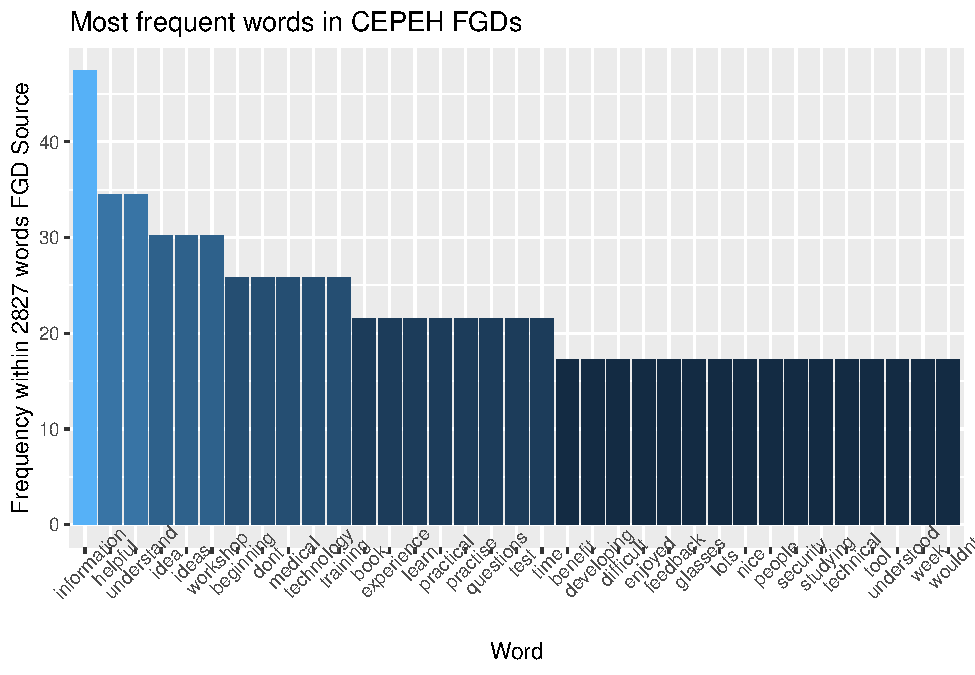
\includegraphics{_main_files/figure-latex/CEPEH MOST FREQ-1} \end{center}

In summary, this understanding of frequent words can help to understand
common concurrences and extrapolate to a larger audience. If scope and
impact of CEPEH chatbots increased we can understand the type of themes
and trends may occur, based on such FGD analysis.

\hypertarget{word-clouds}{%
\section{Word clouds}\label{word-clouds}}

To visualise the most frequent words in another format, below is a word
cloud which presents the word size to indicate the frequency- words that
occur more often being displayed in a larger font size. This has a
normalised data frequency in accordance to the FGD source document
analysed.

\begin{center}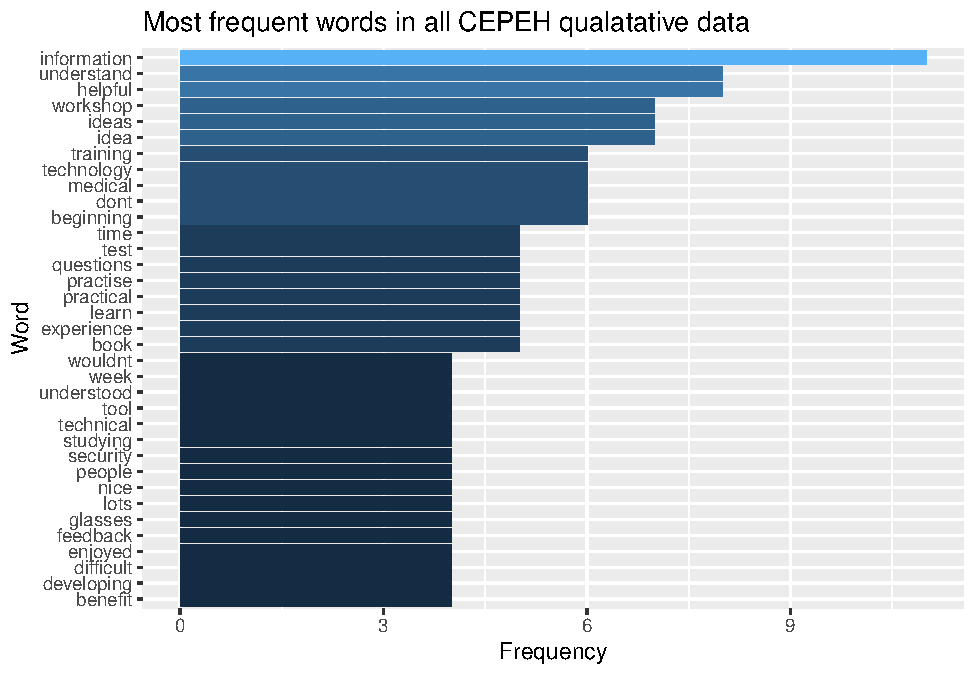
\includegraphics{_main_files/figure-latex/unnamed-chunk-8-1} \end{center}

We understand the context has been reduced for each word. However, in
general there can be categorised positive/negative words from the word
cloud: Positive words are- benefit, practical, nice, helpful, learn,
ideas, and enjoyed Negative words are- difficult, test (who likes a
test?), don't, and `lot' may be negative if there is a `lot' of
information.

\hypertarget{the-vocabulary-of-texts}{%
\subsection{The vocabulary of Texts}\label{the-vocabulary-of-texts}}

Here is a graph that has plotted the words in places depending on the
word frequencies. Additionally, colour hotspots shows how different the
frequencies are - darker items are more similar in terms of their
frequencies, lighter-coloured ones more frequent in one text compared to
the other.

\begin{flushleft}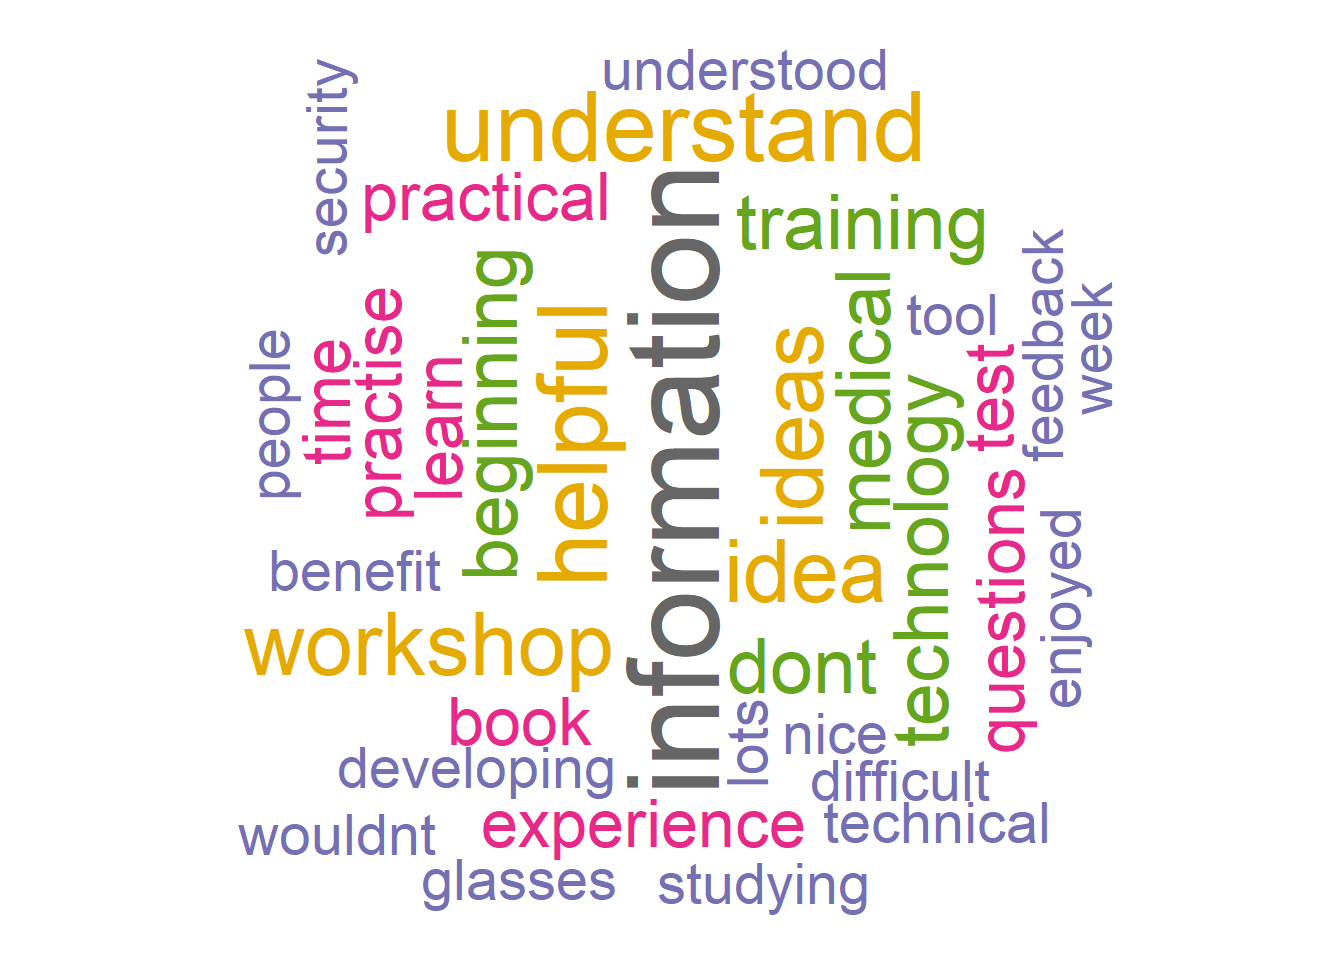
\includegraphics{_main_files/figure-latex/unnamed-chunk-10-1} \end{flushleft}

\hypertarget{sentiment-analysis}{%
\section{Sentiment analysis}\label{sentiment-analysis}}

What is the sentiment of all participants? What is types of emotional
words are being used? The preparation of these words has some use in
understanding the frequencies, but their emotional valence are not
compared. The table above has the word \emph{`helpful'} which has a positive
connotation, however there are 386 words, with many having several
occurrences.

As the table below shows. the FGD data has been analysed for sentiment
of each word, and has been calculated to have 62 positive emotional
valence of words, with 24 negative valence of words. These are from a
\textbf{Bing sentiment lexicon} which is the most popular English language
dictionary.

\begin{tabular}{r|r|r}
\hline
negative & positive & total\_score\\
\hline
24 & 62 & 38\\
\hline
\end{tabular}

Unfortunately, there is little research using sentiment analysis for
chatbot related focus group results that can help to understand the
scoring found. However, on a basic interpretation the higher the score
the better the chatbots were discussed in the FGD's. A score of 72\%
(62/(24+62))) would be in 3/4th quartile in distribution of sentiment
distribution. Alternatively, 62/24 = 2.58 would state the ratio that for
every 1 negative word recorded, there were 2.58 positive words recorded.

\hypertarget{Discussion}{%
\chapter{Discussion}\label{Discussion}}

\minitoc 

\#\#Summary

A quick setup using r git and site pushing just to show basisc skill. thanks

output:
\#bookdown::html\_document2: default
\#bookdown::word\_document2: default
bookdown::pdf\_document2:
template: templates/template.tex
documentclass: book

\hypertarget{cites-and-refs}{%
\chapter{(Additional Analyses) Training Events}\label{cites-and-refs}}

\chaptermark{Citations and cross-refs}

\minitoc 

\hypertarget{cepeh-training-event-c1}{%
\section{CEPEH Training Event C1}\label{cepeh-training-event-c1}}

The CEPEH training event C1 held at the premises of University of Nottingham aiming to prepare participants for the practical elements of co-creation and implementation of chatbots as an educational resource. It combined both theoretical and hands-on training.
15 participants were from RISE, AUTH, UoN.

Project managers of partners signposted the person involved, and relevant announcements were made though social media channels to the wider public. External to the project speakers were from University of Leeds, and Computer Science Department of University of Nottingham. It included academics, medical doctors, and researchers with focus both on clinical research and digital innovations in healthcare education and IT specialist/learning technologists 11.18 years of experiences (SD=7.2). A balance between male and female participants achieved.

Participants were asked to highlight what they liked for each day and how each day can be improved. Findings are described below per day of the training event

Day 1\\
The participants comment that they liked the design method for educational resources presented using a co-creation approach, they liked the interactions with other groups, and they liked the overview of existing chatbot resources of the partners. On the areas that can be improved, more media material were requested.

Day 2
Participants enjoyed the presentation from the invited speaker from another faculty of the University of Nottingham, the CEPEH recources presented and the storyboarding process. Participants highlighted that the participation of more clinicians in the event would be an added value in regards with the storyboarding process.

Day3
Participants liked the hands-on activities of the day also enjoyed the creativity of the groups on the online chatbot development tool. As an area of improvement, participants wanted more time on hands on sections.

\hypertarget{cepeh-training-event-2}{%
\section{CEPEH Training Event 2}\label{cepeh-training-event-2}}

\textbf{Pre-Training Event survey May 9th-13th 2022 Thessaloniki, Greece}

Twenty-six participants attended the Training Event, along with approximately 10 staff members. There were 21 undergraduate students and 5 postgraduate students, who completed the survey for a total of 26 responses. There were 86\% of participants who stated they had not been to a similar event like the training event CEPEH facilitated. There were 90\% of students who found the event schedule very organised, and 70\% agreed most of the planned sessions were relevant to that interest with the remaining 30\% not having enough experience to understand the context to determine if they are interested in the training event. There were 95\% of students agreeing or strongly agreeing the training event location is great, the remaining person did not leave additional comments.

Table 1 suggested attendees had minimal intention to share their own ideas due to lack of previous experience of attending such events, or due to lack of knowledge on the area. However, most were interested in listening to other groups and hearing contextual cases in healthcare.

There were 77\% of participants stated they were novices in experience with chatbots in healthcare and were attending to learn more. The remaining 23\% (7 students) stated they were competent and had limited experience with chatbots in healthcare.

One day had several events regarding cybersecurity in healthcare. When asked before these events, 83\% stated they were neutral or disagreed that they felt confident about their cybersecurity knowledge in healthcare. In addition, 80\% stated they when neutral or disagreed that they felt they had strong cybersecurity safety in healthcare. Table 2 shows the main pre and post results suggesting a positive experience for more than 75\% of attendees on all measures.

There were 90\% (23) of students who heard about the event through a lecturer or a professor, the CEPEH newsletter (2), and 1 person was informed through the anatomy tutoring system at Karolinska Institute. Additionally, 60\% suggested the training event to somebody else before the course started.

There were six individuals who stated neutral or disagree when asked if having issues on registration or finding the information for the event. This may have been due to being dependent on emails to receive the information, instead of a dedicated website where the information is available anytime.

As this was face-to-face, participants were asked about sufficient Covid-19 precautions in place at the facility, 94\% agreed with sufficient precautions, two individuals stated no but did not give further information in the additional input box provided.
In summary, most participants were undergraduate students with novice experience, happy with the training event location, felt the sessions were relevant to them, and most shared the event with their colleagues. The values of co-creation, chatbots in healthcare, and taking patient history were bestowed to students in an engaging and well-received manner. Notably, the highest ratings were for staff friendliness which is key to engagement and consistent interaction throughout the intense and long 5-day duration. The sessions were recorded there for the online recordings may be viewed with higher numbers over the subsequent weeks.

\hypertarget{bibliography-bibliographyreferences.bib-bibliographyadditional-references.bib}{%
\section{\# bibliography: {[}bibliography/references.bib, bibliography/additional-references.bib{]}}\label{bibliography-bibliographyreferences.bib-bibliographyadditional-references.bib}}





\hypertarget{appendix}{%
\chapter*{Appendix}\label{appendix}}
\addcontentsline{toc}{chapter}{Appendix}

\startappendices

\hypertarget{the-first-appendix}{%
\chapter{The First Appendix}\label{the-first-appendix}}

This first appendix includes an R chunk that was hidden in the document (using \texttt{echo\ =\ FALSE}) to help with readability:

\textbf{In 02-rmd-basics-code.Rmd}

\textbf{And here's another one from the same chapter, i.e.~Chapter \ref{code}:}

\hypertarget{references}{%
\chapter*{References}\label{references}}
\addcontentsline{toc}{chapter}{References}

\markboth{References}{}

\hypertarget{refs}{}
\begin{CSLReferences}{1}{0}
\leavevmode\vadjust pre{\hypertarget{ref-Darwin1859}{}}%
Darwin, C. (1859). \emph{{On the Origin of Species by Means of Natural Selection or the Preservation of Favoured Races in the Struggle for Life}}. John Murray.

\leavevmode\vadjust pre{\hypertarget{ref-von_goethe_wilhelm_1829}{}}%
Goethe, J. W. von. (1829). \emph{Wilhelm {Meisters} {Wanderjahre} oder die {Entsagenden}}. Cotta.

\end{CSLReferences}

%%%%% REFERENCES


\end{document}
